\documentclass[11pt]{article}
\usepackage{float}
\usepackage{graphicx}
\usepackage{tabularx}
\usepackage{adjustbox}
\usepackage{amsmath,amssymb,trimclip,adjustbox}
%\usepackage[utf8]{inputenc}
%\usepackage[T1]{fontenc}
\usepackage{textcomp}
\usepackage{booktabs}
\begin{document}
	\begin{titlepage}
		\begin{center}
			\Large{Warsaw University of Technology's}\\
			\Large{Faculty of Mathematics and Information Science}\\
			[0.3in]
			\begin{figure}[H]
				\centering
				
\includegraphics[width=0.4\linewidth, height=0.25\textheight]{./media/uni_logo.jpeg}
				\label{Figure:f04}
			\end{figure}
			\Large{\bfseries Knowledge Representation and Reasoning}\\
			[0.3in]
			\Large{\bfseries Project number 2:}\\
			\Large{\bfseries Deterministic Action With Cost}\\
			\Large{\bfseries Supervisor: Dr Anna Radzikowska}\\
			[0.3in]
			\textsc{\Large{Created By}\\
				Rishabh Jain,
				Rahul Tomer,
				Kuldeep Shankar,\\ 
				Alaa Abboushi,
				Haran Dev Murugan,\\
				Bui Tuan Anh.\\}
		\end{center}	
	\end{titlepage}
	\tableofcontents
	\newpage
	\section{Introduction}\label{sec:intro}
	A dynamic system (DS) is viewed as
	\begin{itemize}
	\item a collection of objects, together with their properties, and
	\item a collection of actions which, while performed, change properties
of objects (in consequence, the state of the world).
	\end{itemize}

	Let C2 be a class of dynamic systems satisfying the following assumptions:
	\begin{enumerate}
		\item Inertia law
		\item Complete information about all actions and fluent. 
		\item Only Determinism
		\item Only sequential actions are allowed.
		\item Characterizations of actions:\begin{itemize}
			\item Precondition represented by set of literals(a fluent or its negation);if a precondition does not hold, the action is executed but with empty effect
			\item Postcondition (effect of an action) represented by a set of literals.
			\item Cost $k \in N $ of an action, actions with empty effects cost 0. Each action has a fixed cost, if it leads to non-empty effects. 
		\end{itemize}
		\item Effects of an action depends on the state where the action starts.
		\item All actions are performed in all states.
		\item Partial description of any state of the system are allowed.
		\item No constraints are defined.	 
	\end{enumerate}
	
	\section{Syntax}\label{sec:syntax}
	
	
	\subsection{Signature :}\label{sec:Signature} 

A signature is a pair $\Upsilon$ = (F, Ac, K) where F is a set of fluents; Ac is a set of actions and K is a set of positive integers representing Cost of each action An $\in$ Ac.

\subsection{Literal :}\label{sec:Literal} 

A literal is either a fluent f or its negation ¬f.\\
\textbf{Notation:} for a fluent f $\epsilon$ F, we write $\overline{f}$to denote the literal corresponding to f, i.e., either f or ¬f.
\subsection{Statements :}\label{sec:Statements} 
	The system and changes occurring within can be described through a sequence of statements defined in the table:
	\begin{table}[H]
  \centering
    \begin{tabular}{|p{2cm}|p{4cm}|p{9cm}|}
    \hline
    \multicolumn{1}{|c|}{\textbf{Statement}} & \multicolumn{1}{c|}{\textbf{Format}} & \multicolumn{1}{c|}{\textbf{Description}} \\
    \hline
    Initial Statement & Initially $\alpha$ holds where $\alpha$ is the initial condition with a set of fluent values. & Initial condition $\alpha$ of the fluent set F$_{\alpha}$ where  F$_{\alpha}$ = \{f1,f2,...,fn\} where  fi $\in$ F and i = 1 to n. \\
    \hline
    Effect Statement & A causes $\alpha$ if g1, . . . , gk & If the action A is performed in any state satisfying g1, . . . , gk, then in
    the resulting state $\alpha$ holds. \\
    \hline
    Value Statement & $\alpha$ after A1 ….An & The condition $\alpha$ always (must) hold after performing the sequence A1 ….An of actions. \\
    \hline
    Cost Statement & A costs C$_{\beta}$, a numerical cost value where C$_{\beta} \in $ K   & If the action A is performed in any satisfying g1, ...,gk then in the resulting state a cost of C$_{\beta}$ is used.C$_{\beta}$ is a numerical value in Cost set K\\
    \hline
    \end{tabular}
    \caption{Syntax Table}
  \label{tab:table01}
\end{table}

	\section{Semantics}
	\begin{itemize}
\item 	A state is a function $\sigma$ : F $\rightarrow$ \{0, 1\}. For any f $\in$ F, if $\sigma$(f) = 1, then we say that f holds in $\sigma$ and write $\sigma$   $\vDash$   f. If $\sigma$(f) = 0, then we write $\sigma$   $\vDash$   ¬f and say that f does not hold in $\sigma$. Let $\sigma$ stand for the set of all states.

\item 	A transition function is a mapping $\Upsilon$ : Ac(K) $\times$ $\sigma$ → $\sigma$. For any $\sigma$ $\in$ $\sum$, for any A $\in$ Ac and for any K$_{i}$ in K, $\Upsilon$(A(K$_{i}$) , $\sigma$) is the state resulting from performing the action A in the state $\sigma$.

\item  In a transition function $\Upsilon$ : A(K$_{i}$) $\times \sigma \rightarrow \sigma$. For any A$_{i} \in$ Ac there exists a cost value K$_{i} \in$ K  where i = 1 to n respectively. 

\item 	A transition function is generalized to the mapping $\Upsilon^{\ast}$ : Ac$^{\ast}$  $\times$  $\sigma$ $\rightarrow$ $\sigma$ as follows: 
$\Upsilon^{\ast}$ ( $\varepsilon$ , $\sigma$) = $\sigma$, $\Upsilon^{\ast}$ ((A1, . . . , An), $\sigma$) = $\Upsilon$(An, $\Upsilon^{\ast}$ (A1, . . . , An-1)).


\item 	Let L be an action language of the class A over the signature $\Upsilon$ = (F, Ac, K). A structure for L is a pair S = ($\Upsilon$, $\sigma_{0}$) where $\Upsilon$ is a transition function and $\sigma_{0}$ $\in$ $\sum$ is the initial state

\item 	Let S = ($\Upsilon$, $\sigma_{0}$) be a structure for L. A statement s$_{\beta}$ is true in S, in symbols S   $\vDash$   s$_{\beta}$, iff s$_{\beta}$ is of the form f after A1, . . . , An, then $\Upsilon$((A1(K$_{1}$), . . . , An(K$_{n}$)), $\sigma_{0}$)   $\vDash$   f; if s$_{\beta}$ is of the form A causes f if g1, . . . , gk and costs K$_{i}$, then for every $\sigma$ $\in$ $\sum$ such that $\sigma$   $\vDash$   gj , j = 1, . . . , k, $\Upsilon$(A(K$_{i}$), $\sigma$)   $\vDash$   f.

\end{itemize}
Let D be an action domain in the language L over the signature $\Upsilon$=(F,A$_{c}$,K). A structure S = ($\Upsilon$,$\sigma_{0}$ is a model of D iff\\
(M1) for every statement s$_{beta}$ $\in$ D, S \textbar= s;\\
(M2) for every Ai $\in$ Ac there exists K$_{i} \in$ K where i = 1 to n, for every f,g1,...,gn $\in$ F, and for every $\sigma\in\sum$, if one of the following conditions holds:
\\\indent
(i) D contains an effect statement\\
\indent\indent 
{\bfseries A causes $\overline{f}$ for the cost value k if} $\overline{g1}$,...,$\overline{gn}$,\\
\indent where k $\neq$ 0 and $\sigma$\textbar=  gi for some i = 1,...,n\\
\indent(ii) D does not contain an effect statement\\
\indent\indent{\bfseries A causes $\overline{f}$ if} g1,...,gn\\
\indent then $\sigma$ \textbar$\neq$ gi iff $\Psi$(A(k),$\sigma$) \textbar$\neq$ gi for some i = 1,...,n, where k = 0.\\

	\section{Examples}\label{sec:Examples}
	\subsection{Example 01}\label{example:ex01}
	\subsubsection{Description}\label{par:p101}
	Andrew wants to travel by his car to a place.Travelling costs him 50\$ if he uses fuel from the fuel tank of the car.If in case of emergency, Andrew is carrying a bottle of fuel as reserve, which can cost him 50\$ for travelling. buying Fuel costs him 100\$ if both fuel and reserve are empty. and buying causes both his Fuel and Reserve are filled. 
	\subsubsection{Representation}\label{par:p201}
	Initially we have:
	\begin{enumerate}
		\item Fuel
		\item Reserve
	\end{enumerate}
	Travel causes $\neg$fuel if fuel %$\vee$ reserve\\
	Travel causes $\neg$reserve if $\neg$fuel $\vee$ reserve\\
	Buy causes fuel, reserve  if $\neg$ fuel $\vee$ reserve\\
	\subsubsection{Calculation}\label{par:p301}\par
	$\sum$ = $\lbrace$ $\sigma_{0}$,$\sigma_{1}$,$\sigma_{2}$ $\rbrace$\\ \\
	$\sigma_{0}$ = $\lbrace$ fuel, reserve $\rbrace$ \indent $\sigma_{1}$ = $\lbrace$ $\neg$fuel, reserve $\rbrace$\\
	$\sigma_{2}$ = $\lbrace$ $\neg$fuel, $\neg$reserve $\rbrace$ 
	\\ \\
	$\Psi$(Buy,$\sigma_{0}$)=$\sigma_{0}$ \indent $\Psi$(Travel,$\sigma_{0}$)=$\sigma_{1}$\\
	$\Psi$(Buy,$\sigma_{1}$)=$\sigma_{1}$ \indent $\Psi$(Travel,$\sigma_{1}$)=$\sigma_{2}$\\
	$\Psi$(Buy,$\sigma_{2}$)=$\sigma_{1}$ \indent $\Psi$(Travel,$\sigma_{2}$)=$\sigma_{2}$\\
	\subsubsection{Graph}\label{par:p401}
	\begin{figure}[H]
		\centering
		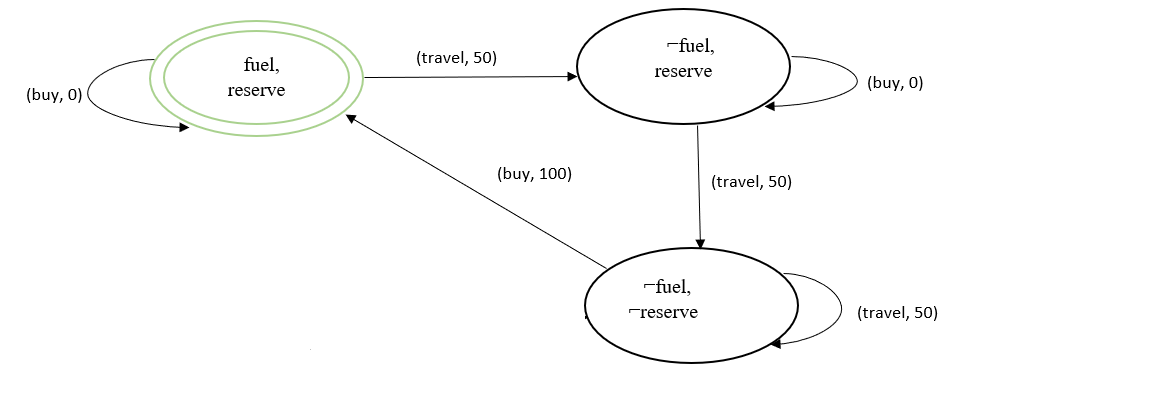
\includegraphics[width=6in,height=3in]{./media/ex01.png}
		\label{Figure:f01}
		\caption{Example 01}
	\end{figure}
	\subsection{Example 02}\label{example:ex02}
	\subsubsection{Description}\label{par:p102}
	John visits a painter to buy a specific painting. The cost of painting is 200\$ if its available in the shop. But if painting is not available then John needs to order a new one to be painted and will buy once its available. At any time only one copy of painting is available and another one to be ordered once sold. 
	
	\subsubsection{Representation:}\label{par:p202}
	\indent 
	\par Fluents: available, sold.\par
	Actions: BUY, ORDER.\par
	BUY costs 200$\$$  \textbf{if} available\par
	
	BUY costs 0$\$$  \textbf{if} ¬available\par
	
	
	Order Cost: 0 $\$$
	
	initially: ¬available $\wedge$  ¬sold\par
	
	BUY causes sold if available\par
	
	ORDER causes available if ¬available\par
	
	BUY causes ¬available\\
	
	\subsubsection{Calculation:}\label{par:p302}
	\indent \par
	$ \sum $ = $ \{ $ $ \sigma $0, $ \sigma $1, $ \sigma $2, $ \sigma $3$ \} $ \par
	
	$ \sigma $0 = $ \{ $ ¬available, ¬sold$ \} $ \par
	
	$ \sigma $1 = $ \{ $ ¬available, sold$ \} $ \par
	
	$ \sigma $2 = $ \{ $ available, ¬sold$ \} $ \par
	
	$ \sigma $3 = $ \{ $ available, sold$ \} $ \par
	\(  \Psi  \)  (BUY, $ \sigma $0) = $ \sigma $0\par
	
	\(  \Psi  \)  (ORDER, $ \sigma $0) = $ \sigma $1\par
	
	\(  \Psi  \)  (BUY, $ \sigma $1) = $ \sigma $2\par
	
	\(  \Psi  \)  (ORDER, $ \sigma $1) = $ \sigma $1\par
	
	\(  \Psi  \)  (BUY, $ \sigma $2) = $ \sigma $2\par
	
	\(  \Psi  \)  (ORDER, $ \sigma $2) = $ \sigma $1\par
	
	\(  \Psi  \)  (BUY, $ \sigma $3) = $ \sigma $2\par
	
	\(  \Psi  \)  (ORDER, $ \sigma $3) = $ \sigma $3\par
	\subsubsection{Graph}\label{par:p402}
	\begin{figure}[H]
		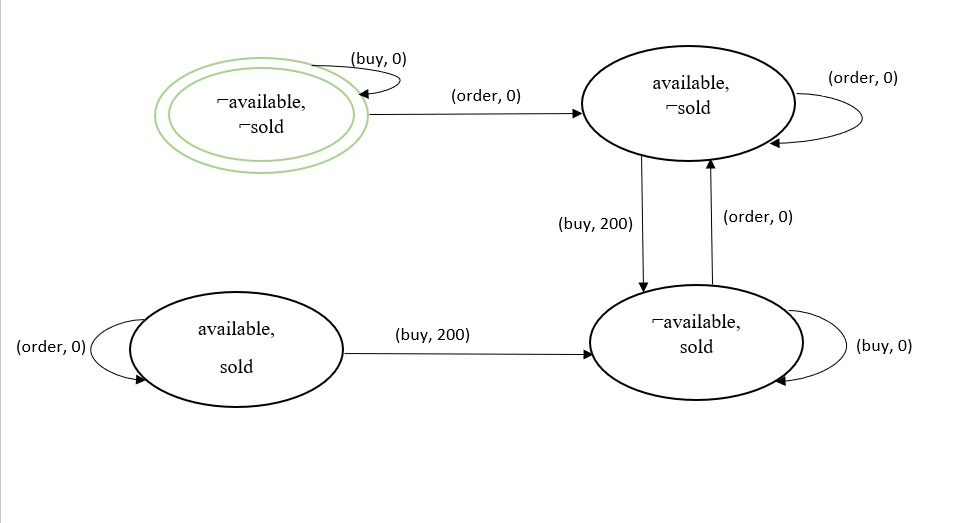
\includegraphics[width=1\linewidth, height=0.4\textheight]{./media/image1.jpeg}
		\label{Figure:f02}
		\caption{Example 02}
	\end{figure}
	\subsection{Example 03}
	\subsubsection{Description}\label{par:p103}
	There is a man. He can cook, eat, and play. Cooking makes food cooked. he can eat food if it is cooked. After eating he feels not hungry, and food is not cooked again. He can play. Playing makes him hungry. He just can play if he is not hungry. He just cooks when there is no food is cooked. Initially, he is hungry, and no food is cooked. In terms of energy, eating costs 5, cooking costs 15, playing costs 20.\\
	\\
	\subsubsection{Representation in language}\label{par:p203}
	Fluents: cooked, hungry.\\
	Actions: cook, eat, play.\\
	\\
	\\
	eat cost 5\\
	cook cost 15\\
	play cost 20\\
	initially $\neg$cooked $\land$ hungry\\
	cook causes cooked if $\neg$cooked\\
	eat causes ($\neg$cooked $\land$ $\neg$hungry) if cooked\\
	play causes hungry if $\neg$hungry\\
	\\
	\subsubsection{Calculation}\label{par:p303}
	$\sum$ = \{$\sigma_{0}$ ,$\sigma_{1}$, $\sigma_{2}$, $\sigma_{3}$\}\\
	\\
	$\sigma_{0}$ = \{$\neg$cooked, hungry\}\\
	$\sigma_{1}$ = \{cooked, hungry\}\\
	$\sigma_{2}$ = \{$\neg$cooked, $\neg$hungry\}\\
	$\sigma_{3}$ = \{cooked, $\neg$hungry\}\\
	\\
	$\psi$(eat, $\sigma_{0}$) = $\sigma_{0}$\\
	$\psi$(cook, $\sigma_{0}$) = $\sigma_{1}$\\
	$\psi$(play, $\sigma_{0}$) = $\sigma_{0}$\\
	\\
	$\psi$(eat, $\sigma_{1}$) = $\sigma_{2}$\\
	$\psi$(cook, $\sigma_{1}$) = $\sigma_{1}$\\
	$\psi$(play, $\sigma_{1}$) = $\sigma_{1}$\\
	\\
	$\psi$(eat, $\sigma_{2}$) = $\sigma_{2}$\\
	$\psi$(cook, $\sigma_{2}$) = $\sigma_{3}$\\
	$\psi$(play, $\sigma_{2}$) = $\sigma_{1}$\\
	\\
	$\psi$(eat, $\sigma_{3}$) = $\sigma_{2}$\\
	$\psi$(cook, $\sigma_{3}$) = $\sigma_{3}$\\
	$\psi$(play, $\sigma_{3}$) = $\sigma_{1}$\\
	\\
	\subsubsection{Graph}\label{par:p403}
	\begin{figure}[H]
		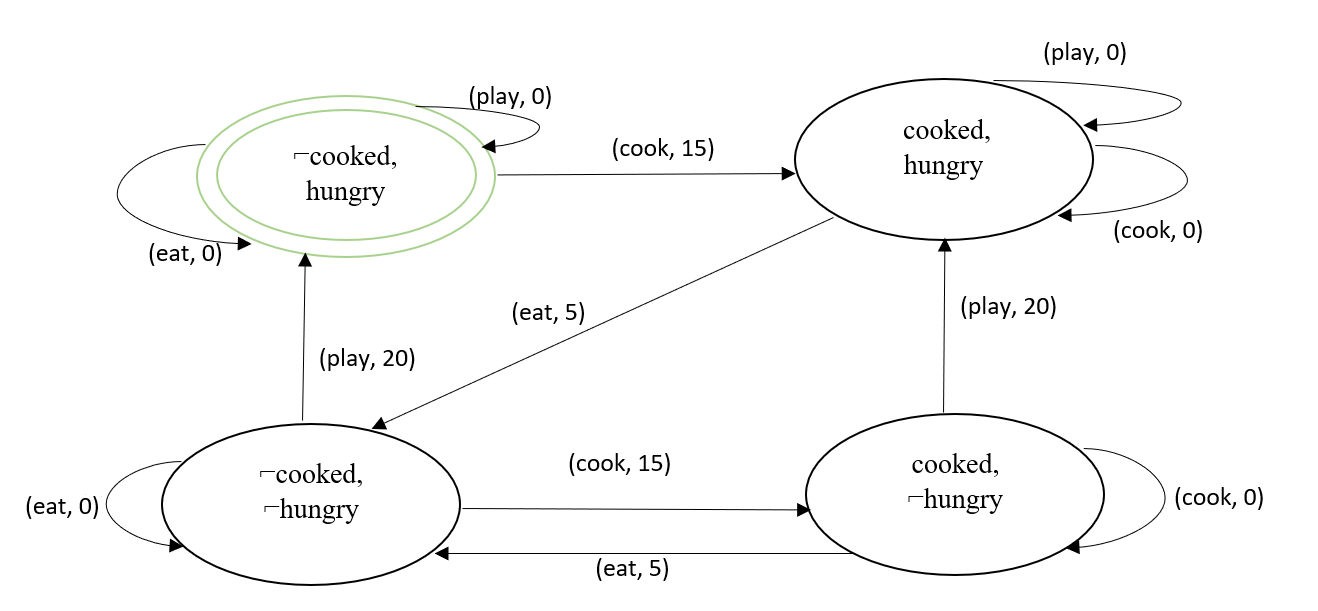
\includegraphics[width=1\linewidth, height=0.3\textheight]{./media/figure01.png}
		\caption{Example 03}
		\label{Figure:f03}
	\end{figure}
	\newpage
	\section{Appendix}	
	\begin{appendix}
		\listoffigures
		\listoftables
	\end{appendix}
\end{document}